% ======================================================================
% GiTrip Project Management Report
% Author: Tatsunori Ono
% Degree/Year: 3rd Year Computer Science
% Supervisor: Professor Mike Joy
% Academic Year: 2025/26
%
% Based on the University of Warwick CS Report Template
% Original template by Chris Quinn 28/06/2020
% ======================================================================

\documentclass[pdftex,11pt,a4paper,oneside]{article}

% -- Original Warwick template packages ----------------------------------
\usepackage{amsmath}
\usepackage{fancyhdr}
\usepackage{graphicx}
\usepackage{setspace}           % Spacing (used on front page for crest)
\usepackage[]{fncychap}         % Section heading style
\usepackage[hyphens]{url}
\usepackage{xcolor}
\usepackage{tabularx}
\usepackage{appendix}
\usepackage{cite}               % IEEE citation grouping [1]-[3]

% -- Additional packages for content -------------------------------------
\usepackage[a4paper,margin=2.5cm]{geometry}
\usepackage{microtype}
\usepackage{lmodern}
\usepackage{booktabs}
\usepackage{array}
\usepackage{float}              % [H] placement for figures
\usepackage{caption}
\usepackage{subcaption}

% Keep hyperref last
\usepackage[hidelinks]{hyperref}

% -- Paragraph formatting ------------------------------------------------
\setstretch{1.15}
\setlength{\parskip}{0.35em}
\setlength{\parindent}{0pt}

% -- Warwick-style header/footer -----------------------------------------
\fancyhf{}
\pagestyle{fancy}
\renewcommand{\headrulewidth}{0.2pt}
\lfoot{\centering \thepage}

%%%%%%%%%%%%%%%%%%%%%%%%%% DOCUMENT STARTS %%%%%%%%%%%%%%%%%%%%%%%%%%%%%

\begin{document}

% ========================================================================
% TITLE PAGE
% ========================================================================
\thispagestyle{empty}

\begin{spacing}{2}
    \begin{center}
        
\includegraphics[scale=0.45]{Preamble/WarwickCrest.pdf}
        % Two options: WarwickCrest.pdf (colour) or WarwickAlt.pdf (B&W)
    \end{center}
    \vspace{5mm}
    \begin{center}
        \textbf{\begin{LARGE}
        GiTrip \\ $\sim$\textit{Git} for Collaborative Trip Planning$\sim$
        \end{LARGE}}
        \vspace{5mm}
    \end{center}
    \begin{center}
        {\large CS310 Computer Science Project}\\
        {\large Project Management Report}
        \vspace{20mm}
    \end{center}
    \begin{center}
        \textbf{\large Tatsunori Ono}
        \vspace{20mm}
    \end{center}
    \begin{center}
        {\large Supervisor: Professor Mike Joy}\\
        \vspace{5mm}
        \textbf{\large Department of Computer Science}\\
        {\large University of Warwick}\\
        {\large Academic Year 2025/26\\}
    \end{center}
\end{spacing}

% ========================================================================
% FRONT MATTER
% ========================================================================
\pagenumbering{roman}

\pagebreak

\tableofcontents

\newpage

% ========================================================================
% MAIN BODY
% ========================================================================
\pagenumbering{arabic}

\section{Introduction}

This report documents the project management of GiTrip, complementing the
Final Report's technical content with evidence of planning, execution, and
reflective practice.

\section{Development Methodology}
\label{sec:methodology}

The project adopted an \emph{iterative waterfall} approach combining three principles: 
\begin{enumerate}
    \item \textbf{Risk-driven prototyping}, where early prototypes validated feasibility of snapshot storage, server-rendered User Interface (UI), and routing integration.
    \item \textbf{Incremental feature delivery aligned to MoSCoW (Must/Should/Could/Won't)}, where Must-haves were implemented first to reach an end-to-end Minimum Viable Product (MVP) before Should-haves and hardening.
    \item \textbf{Continuous feedback} through regular supervisor meetings (Term~1 Weeks 1, 2, 4, 5, 7, 9; Term~2 Weeks 1, 2, 4, 6, 8, 10).
\end{enumerate}
Milestones remained stable to match university deadlines (Project Specification, Progress Report, Evaluation Day, final submission), while work within each milestone was refined through short feedback cycles. For example, Application Programming Interface (API) quota exhaustion in Term~1 Week~7 prompted immediate caching and fallback implementation. This maps onto a conventional software life cycle~\cite{ref_sommerville} but revisited earlier phases when feedback demanded it (e.g., the merge engine was revised three times), retaining milestone-driven predictability while incorporating iterative adaptability~\cite{ref_sommerville}.

Early work consisted of competitor analysis, literature review, and a preliminary survey (November 2025), producing the Project Specification, MoSCoW objectives, and an evaluation plan.

\section{Time Management and Work Tracking}
Time management combined a Gantt-style plan with weekly goal-setting and review.
The plan was organised around Term~1 delivery of the end-to-end MVP and Term~2 hardening (tests, robustness, deployment, and evaluation
readiness). Weekly work was prioritised using MoSCoW,
protecting Must-have items first.

\begin{table}[H]
\centering
\caption{Milestone plan (summary).}
\label{tab:milestones}
\begin{tabular}{@{}p{0.22\linewidth}p{0.68\linewidth}@{}}
\toprule
\textbf{Period} & \textbf{Primary deliverables} \\
\midrule
Nov--Dec 2025  & Research, survey, Project Specification, initial prototypes \\
Dec 2025--Jan 2026 & Repository model, planner pipeline, editing UI, initial
                     merge workflow \\
Feb 2026       & Hardening, automated tests, deployment, evaluation preparation \\
Late Feb 2026  & Evaluation Day demonstration and data collection \\
Mar 2026       & Final integration and documentation \\
\bottomrule
\end{tabular}
\end{table}

Progress was monitored using three artefacts:
\begin{enumerate}
  \item \textbf{Supervision notes:} each meeting used a prepared agenda recorded
        in Obsidian~\cite{ref_obsidian} with a structure inspired by the Cornell note-taking
        system~\cite{ref_cornell}, splitting the note into three sections:
        ``Updates from Last Meeting and General Notes'', ``Questions to Ask and
        Answers'', and ``To-dos and Summary''. Whenever questions arose between
        meetings, they were recorded in the ``Questions to Ask'' section of the
        next meeting file. Notes were additionally backed up via an automated
        GitHub~\cite{ref_github} plugin sync (every 15 minutes) to reduce the risk of data loss,
        as shown in Appendix~\ref{appx:github-backup}. A sample meeting
        note demonstrating this structure is included in
        Appendix~\ref{appx:meeting-note}.
  \item \textbf{Source control history:} all work was committed to GitHub for
        backup and traceability. By completion the repository contained over
        200 commits across multiple feature branches
        (Figure~\ref{fig:github-commits}).
  \item \textbf{Living schedule:} the original Gantt chart from the Project
        Specification was reviewed weekly. When a three-day delay emerged due to
        API quota exhaustion, the timetable was revised to absorb the delay
        through buffer time and tasks were re-prioritised.
\end{enumerate}


\begin{figure}[H]
  \centering
  \includegraphics[width=0.92\linewidth]{Figures/github-commits.png}
  \caption{GitHub contribution heatmap for 2025--2026. This shows the author's
           overall GitHub activity; GiTrip development accounts for the
           majority of contributions from August 2025 onwards. Contributions
           span multiple GiTrip repositories as the project was restructured
           across iterations.}
  \label{fig:github-commits}
\end{figure}

Figure~\ref{fig:gantt-updated} shows the updated Gantt chart reflecting the
actual project timeline. The original Gantt chart from the Progress Report is
included in Appendix~\ref{appx:original-gantt} for comparison.

\begin{figure}[H]
  \centering
  \includegraphics[width=\textwidth]{Figures/gantt-final.png}
  \caption{Updated Gantt chart showing the final project timeline with completed status for all phases in Terms~1 and 2.}
  \label{fig:gantt-updated}
\end{figure}

\begin{figure}[H]
  \centering
  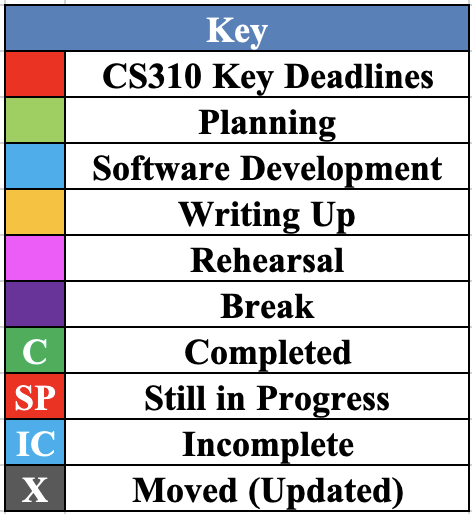
\includegraphics[width=0.25\textwidth]{Figures/gantt-key.png}
  \caption{Gantt chart keys with status indicators.}
  \label{fig:gantt-key}
\end{figure}

Table~\ref{tab:milestone-comparison} compares planned versus actual completion dates, updated from the Progress Report to include Term~2.

\begin{table}[H]
\centering
\begin{tabularx}{\textwidth}{c X c c c}
\toprule
\textbf{\#} & \textbf{Milestone} & \textbf{Planned} & \textbf{Actual} & \textbf{Status}\\
\midrule
4 & Project Specification (Formative) & Oct 16 & Oct 15 & Complete\\
5 & User Experience (UX) flows and wireframes & Mid Oct & Mid Oct & Complete\\
6 & Seed data, data model, migrations & Late Oct & Late Oct & Complete\\
7 & Commit, branch, merge operations & Late Oct & Late Oct & Complete\\
8 & Place search via proxy & Late Oct & Late Oct & Complete\\
9 & Nearest Neighbour (NN) ordering \& constraints algorithm & Late Oct--Early Nov & Late Oct--Early Nov & Complete\\
10 & Opening-hours ingestion \& parsing & Mid Nov & Late Jan & Complete\\
11 & API Reliability hardening & Mid Nov & Mid Nov & Complete\\
12 & OpenRouteService (ORS)/Google routing integration & Mid Nov & Mid Nov & Complete\\
13 & Multi-day spillover & Mid Nov & Mid Nov & Complete\\
14 & Compact vs.\ sparse & Mid Nov & Mid Nov & Complete\\
15 & Focus-time preference & Late Nov & Late Nov & Complete\\
16 & Desired time windows & Late Nov & Late Nov & Complete\\
17 & Strict ordering/start pin & Early Dec & Early Dec & Complete\\
18 & Recompute travel by mode & Early Dec & Early Dec & Complete\\
19 & Conflict resolver per stop/field & Early Dec & Late Jan & Complete\\
20 & Commit edits from timeline/map & Early Dec & Early Dec & Complete\\
21 & Progress Report & Jan 22 & Jan 21 & Complete\\
22 & Progressive Web App (PWA) & Late Jan & Early Jan & Complete\\
23 & Security check & Late Jan & Early Dec & Complete\\
24 & Automated tests (unit \& merge) & Feb & Feb & Complete\\
25 & Evaluation Day & Late Feb & Feb 25 & Complete\\
26 & Final Report \& submission & Late Mar & Late Mar & Complete\\
\bottomrule
\end{tabularx}
\caption{Planned vs.\ actual milestone completion (Terms~1 and~2).}
\label{tab:milestone-comparison}
\end{table}

To sustain momentum, each week ended with an integrated build and a short review against the schedule, recording what was completed and what slipped. This ensured that demonstrations for supervision and Evaluation Day were always based on the current main branch.

\section{Stakeholder Management}
The key stakeholder was the supervisor, Professor Mike Joy, with whom 12 meetings were held across both terms using the Cornell-inspired Obsidian notes described in Section~\ref{sec:methodology}. Each meeting followed a repeatable process: before the meeting, progress updates and questions were prepared; during the meeting, responses were noted beside each item; afterwards, action items were summarised and converted into the next week's tasks. This structured approach reduced rework by systematically organising outstanding tasks.

Due to the author's course transfer from MEng to BSc Computer Science, the
supervision meeting recordings on Tabula are split across two pages
(Figures~\ref{fig:tabula-bsc} and~\ref{fig:tabula-meng}).

\begin{figure}[H]
  \centering
  
\includegraphics[width=0.85\linewidth]{Figures/tabula-1.png}
  \caption{Dissertation supervisor record of meetings on Tabula (BSc page).}
  \label{fig:tabula-bsc}
\end{figure}

\begin{figure}[H]
  \centering
  
\includegraphics[width=0.85\linewidth]{Figures/tabula-2.png}
  \caption{Dissertation supervisor record of meetings on Tabula (MEng page).}
  \label{fig:tabula-meng}
\end{figure}

Feedback from the Progress Report assessment was incorporated into Term~2
planning. Concerns about overly complex diagrams informed a decision to use
smaller, purpose-specific figures in the Final Report. The second assessor's
suggestion to explore machine learning was recorded as future work without
expanding the MVP scope.

\section{Risk Management and Resilience}
A lightweight risk register was maintained and revisited during supervision.
Table~\ref{tab:risk} lists the most significant risks, mitigations, and outcomes.

\begin{table}[H]
\centering
\caption{Key risks and mitigations.}
\label{tab:risk}
\begin{tabular}{@{}p{0.24\linewidth}p{0.34\linewidth}p{0.32\linewidth}@{}}
\toprule
\textbf{Risk} & \textbf{Mitigation} & \textbf{Outcome} \\
\midrule
External routing API failure / quota limits
  & Caching, rate limiting, bounded concurrency, Haversine fallbacks
  & Planner remained usable and demos remained reliable. \\
\midrule
Merge correctness (silent data loss)
  & Merge hardening plus 16 unit tests for conflicts and deletions
  & Merge behaviour became deterministic and test-backed. \\
\midrule
Git concepts confusing for novices
  & Easy mode toggle; seeded demos; clearer labels and affordances
  & Most users completed key tasks; issues logged for future work. \\
\midrule
Data loss (notes or DB)
  & GitHub backups; Obsidian sync; persistent SQLite volume on Fly.io
  & Reduced single points of failure. \\
\midrule
Evaluation logistics (network, devices)
  & Public deployment (Fly.io) and multi-device setup
  & Four Linux machines plus laptop; attendees also used personal devices. \\
\bottomrule
\end{tabular}
\end{table}

Evaluation risk was reduced by preparing a seeded merge-conflict repository and a Microsoft Forms survey for consistent feedback collection.

\section{Unforeseen Issues and How They Were Handled}
Several unforeseen issues required adaptation:

\textbf{API quota exhaustion.} OpenRouteService rate limits were hit during intensive testing, causing the planner to return errors. A Time-To-Live (TTL) cache, bounded concurrency (maximum four simultaneous requests), and Haversine fallback were added so the planner degrades gracefully rather than failing entirely. The schedule adjustment was absorbed by buffer time.

\textbf{Merge edge cases.} \texttt{JSON.stringify}-based comparison produced false positives when key ordering differed between branches. The merge engine was reworked to use deep structural equality and stable stop identifiers, completed before Evaluation Day and backed by 16 automated tests.

\textbf{Place search typo sensitivity.} Nominatim's exact index matching meant near-miss queries (e.g.\ ``stick n sushi'' for ``Sticks'n'Sushi'') returned no results. Adding Photon as a fuzzy-search fallback resolved this using the same OpenStreetMap data with typo-tolerant indexing.

\textbf{Constraint-aware interactive editing.} Timeline drag-and-drop could produce invalid plans. A two-tier strategy was adopted: UI-level constraint enforcement with visual feedback, and server-side feasibility checks on commit.

\textbf{Increased operational work.} Deployment hardening (security headers, Content Security Policy (CSP), HTTPS, rate limiting) and Fly.io deployment were not originally scoped but proved necessary for reliable demonstrations. The boundary excluding generative Artificial Intelligence (AI) remained unchanged to avoid scope creep.

\section{Legal, Ethical, Social and Professional Issues}

\subsection{Ethical Consent and Human Participation}
Two activities involved human participants: a preliminary survey (November 2025, 30 responses) and Evaluation Day user acceptance testing (February 2026, 13 responses). Both were low-risk; responses were collected anonymously via Microsoft Forms and reported in aggregate. Formal ethical approval was not required, but good practice was followed: minimal data collection, no sensitive questions, and the ability to withdraw. If GiTrip were to become a commercial product, a more robust study with formal consent procedures (information sheet, explicit consent, and clearer withdrawal mechanisms) would be required.

\subsection{Data Protection and Privacy}
GiTrip stores only essential identifiers (email, username) with bcrypt-hashed passwords. Session cookies are HttpOnly/SameSite=Lax, and access control uses visibility settings and collaborator roles. The design aligns with General Data Protection Regulation (GDPR) principles~\cite{ref_gdpr}.

\subsection{Third-Party Services and Legal Compliance}
GiTrip integrates with OpenStreetMap, Nominatim, Photon, OpenRouteService, Google Directions, GNews, and Open-Meteo. Usage policies were respected through caching, rate limiting, and bounded concurrency; attribution is displayed in the UI~\cite{ref_osm_tiles} and API keys are never exposed to clients.

\subsection{Accessibility}
Accessibility followed Web Content Accessibility Guidelines (WCAG)~2.2~\cite{ref_wcag22}, providing font-size adjustment, high-contrast mode, and read-aloud mode (Figure~\ref{fig:accessibility}). Remaining limitations (map and timeline drag controls) are documented in the Final Report.

\begin{figure}[H]
  \centering
  \begin{subfigure}[t]{\linewidth}
    \centering
    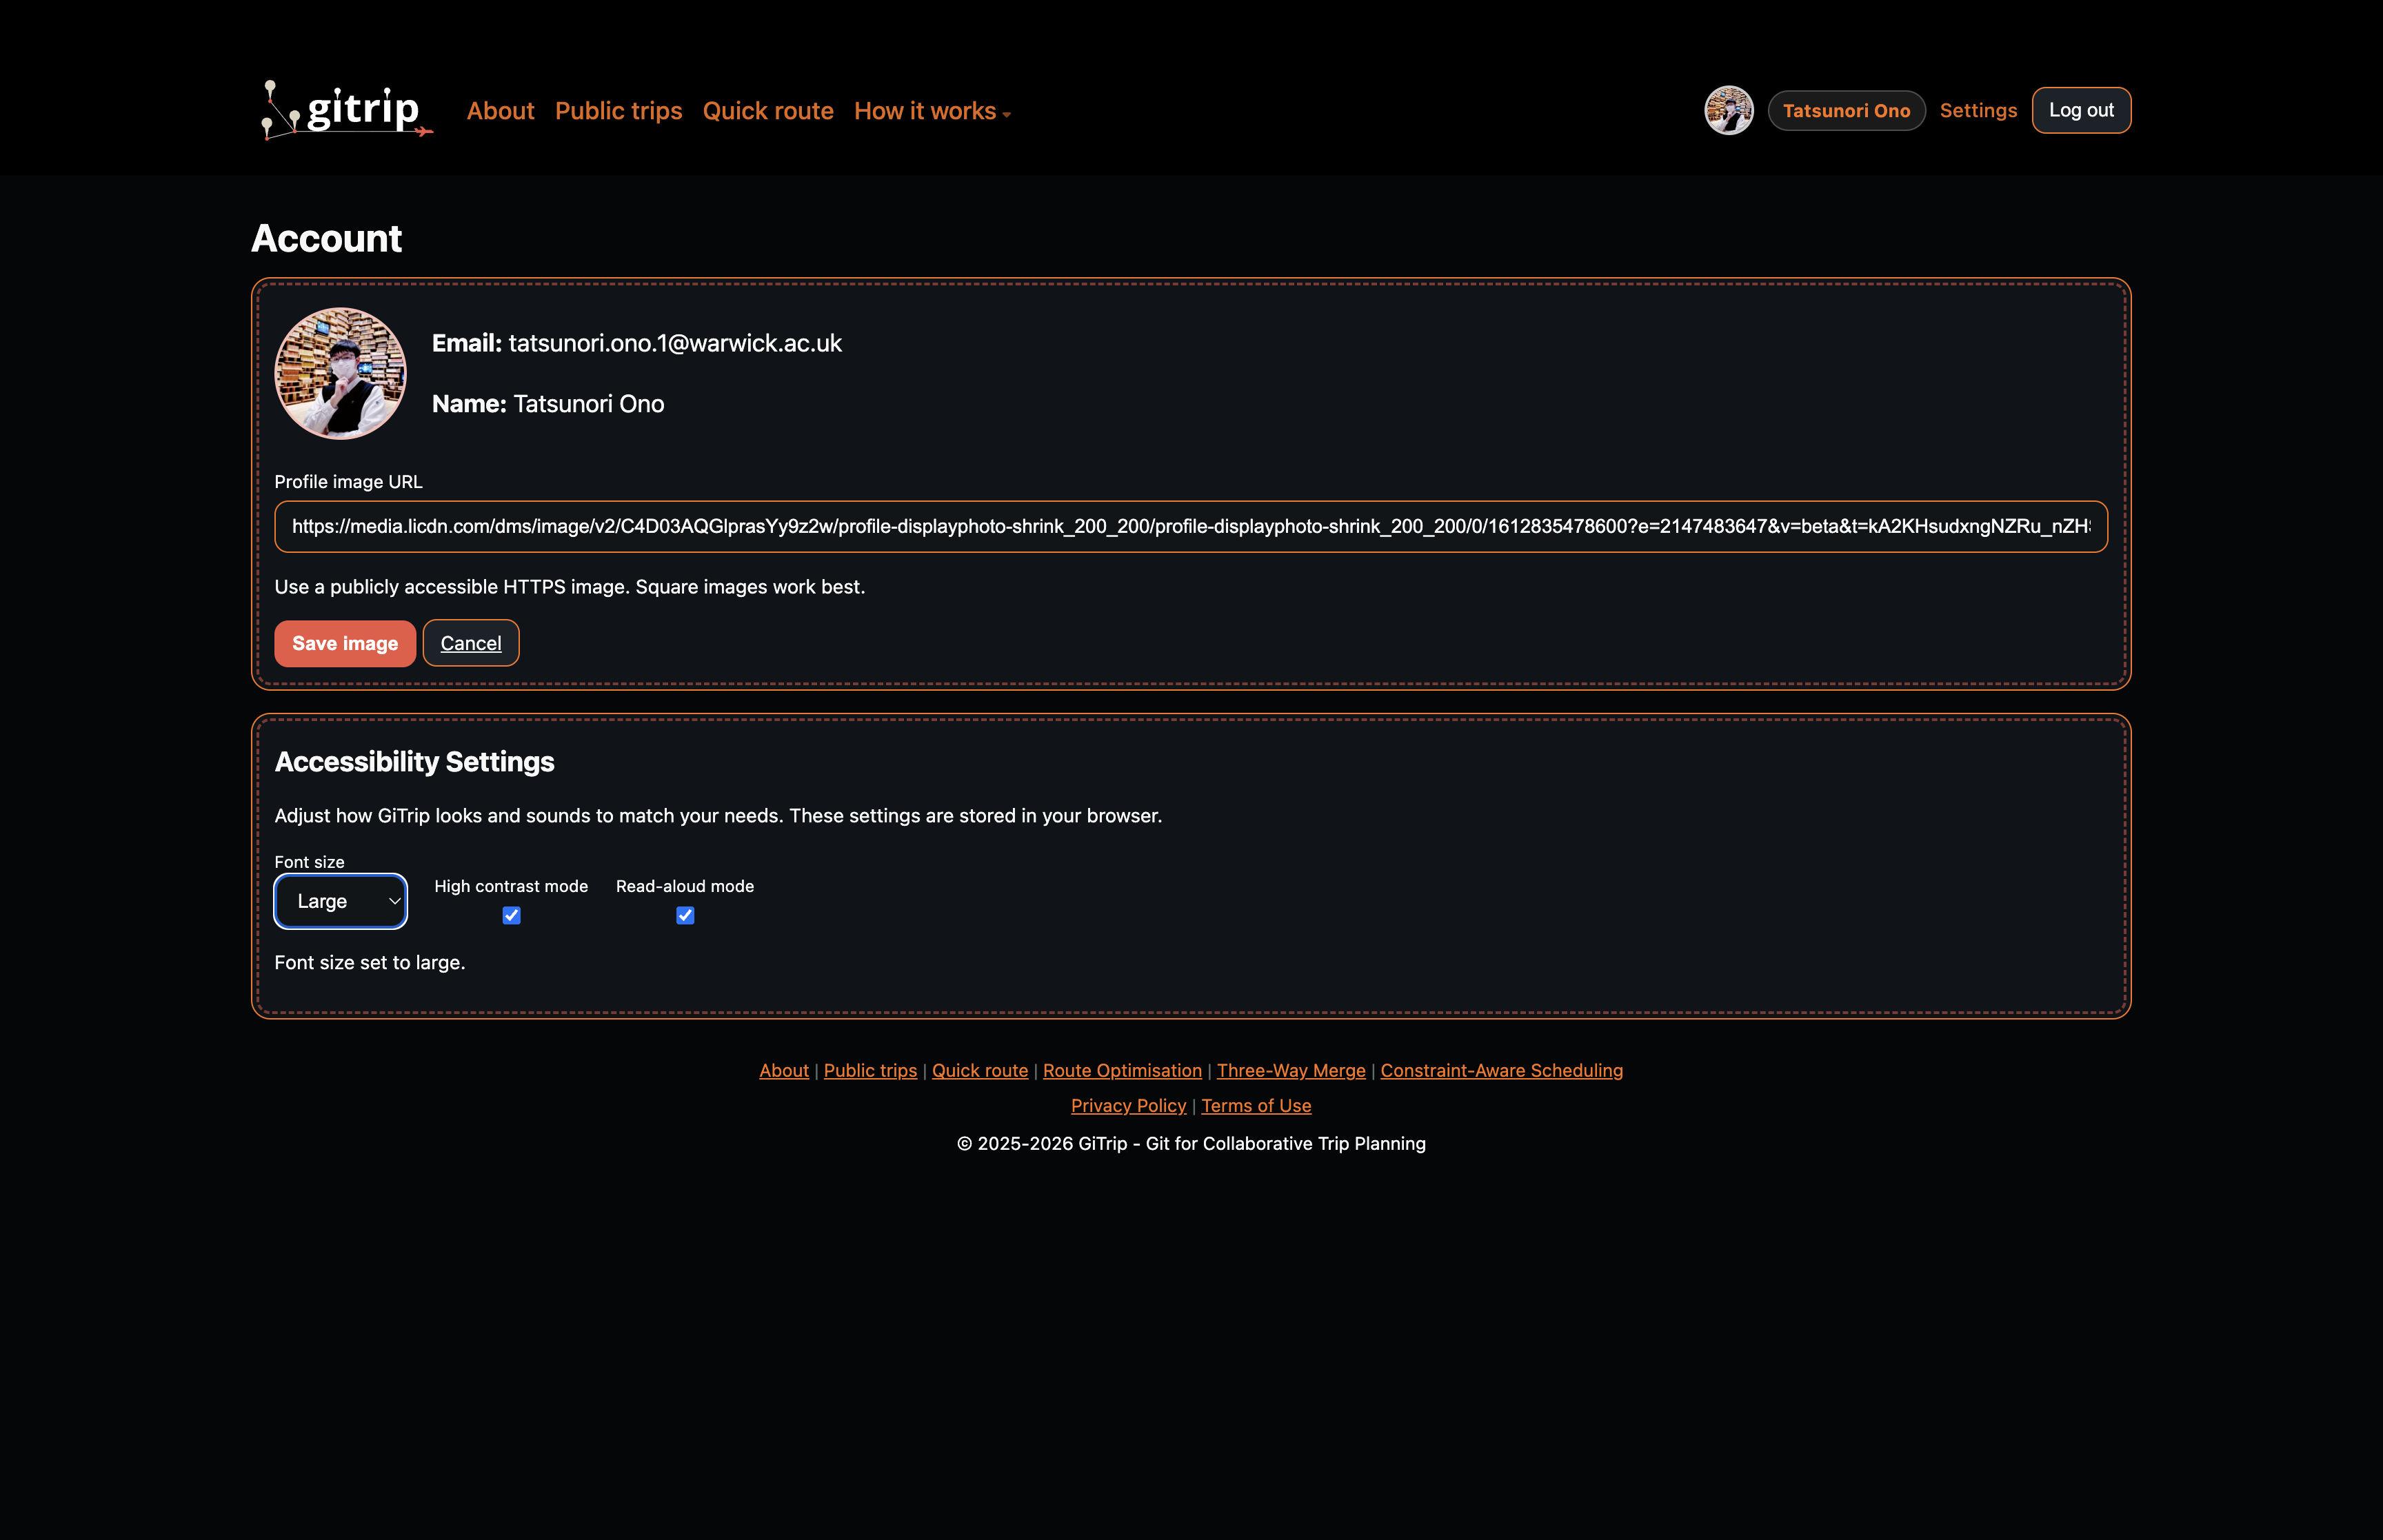
\includegraphics[width=0.85\linewidth]{Figures/ui-accessibility-1.png}
    \caption{Settings panel for accessibility options.}
  \end{subfigure}

  \vspace{0.5em}
  \begin{subfigure}[t]{\linewidth}
    \centering
    \includegraphics[width=0.85\linewidth]{Figures/ui-accessibility-2.png}
    \caption{Quick explore page with high-contrast, read-aloud mode, and large font enabled.}
  \end{subfigure}
  \caption{Accessibility features: font-size adjustment, high-contrast mode,
  and read-aloud mode.}
  \label{fig:accessibility}
\end{figure}

\subsection{Professional Conduct}
Professional behaviour followed the BCS Code of Conduct~\cite{ref_bcs}: honest reporting of results including limitations, proper attribution, and transparent documentation of scope boundaries.

\section{Conclusion}
GiTrip was delivered through milestone-driven execution and iterative refinement under regular supervision. Risks were mitigated through fallbacks, testing, and scope control, with attention to ethics, privacy, legal compliance, and accessibility.

% ========================================================================
% REFERENCES (IEEE style)
% ========================================================================
\addcontentsline{toc}{section}{References}
\bibliographystyle{ieeetr}
\bibliography{bibliography}

% ========================================================================
% APPENDIX
% ========================================================================
\begin{appendices}

\section{Original Gantt Chart (Progress Report)}
\label{appx:original-gantt}

The following Gantt chart was included in the Progress Report, showing the
planned and actual progress at the end of Term~1. It is reproduced here for
comparison with the updated timeline in the main body
(Figure~\ref{fig:gantt-updated}).

\begin{figure}[H]
  \centering
  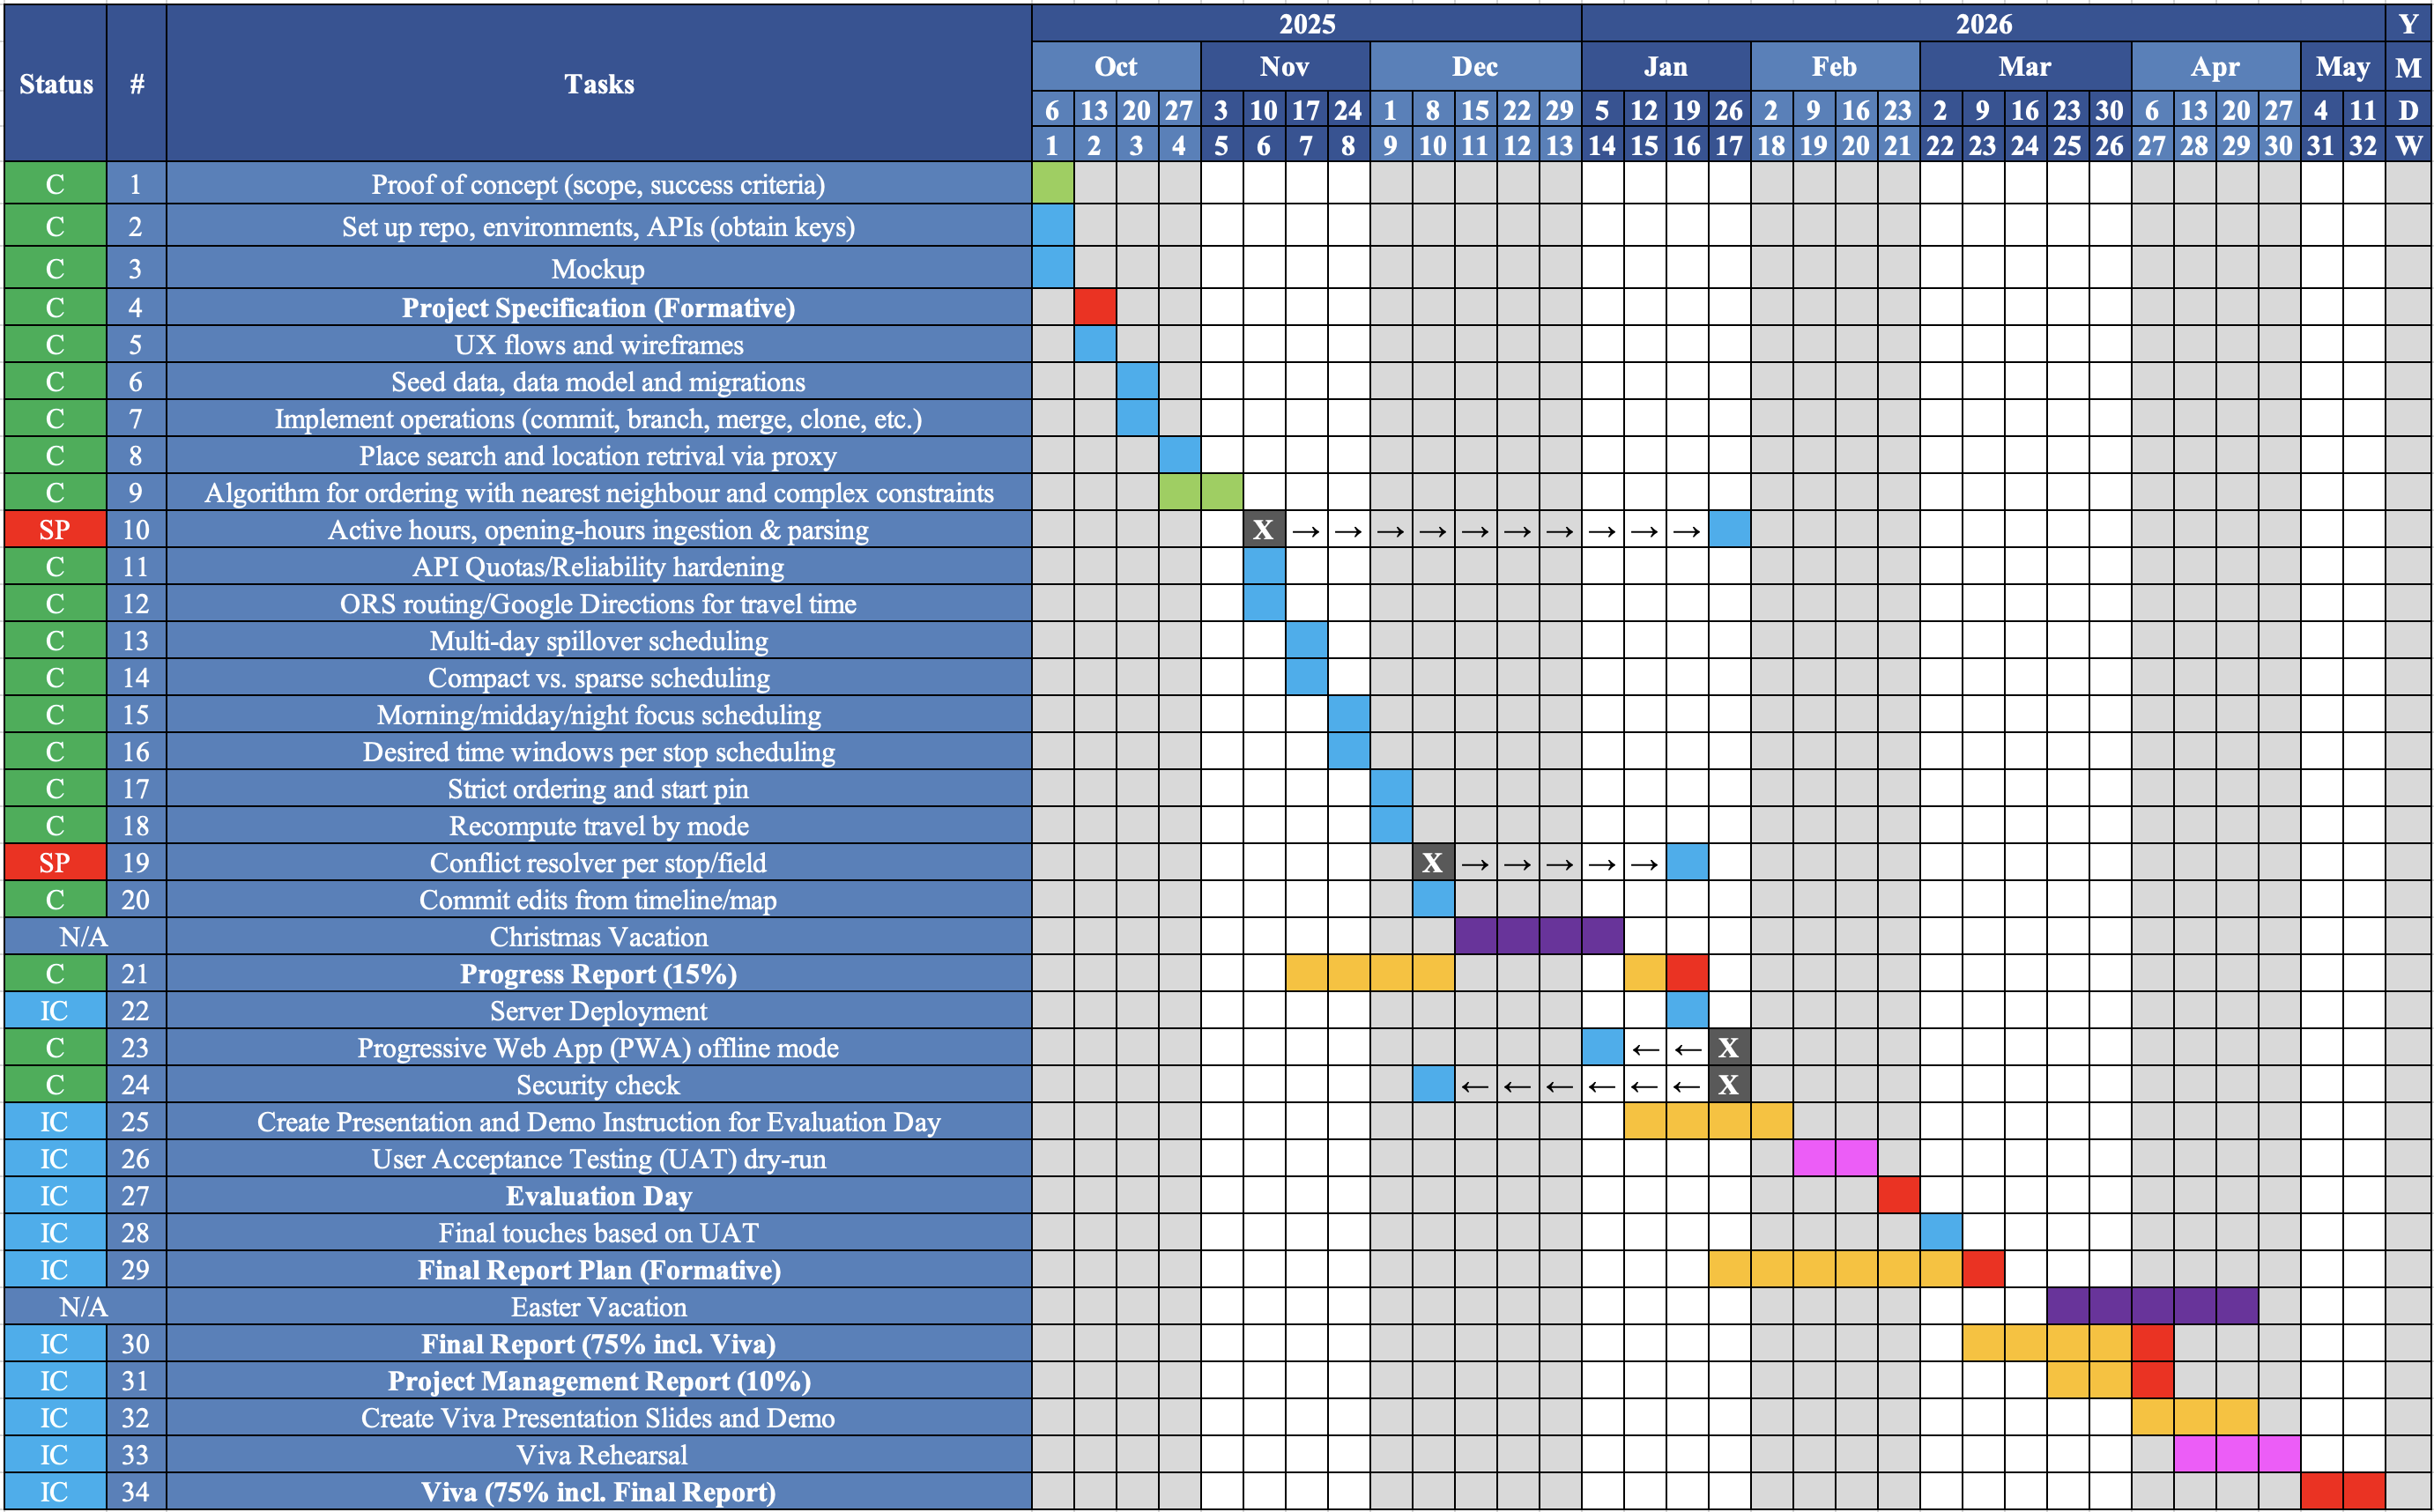
\includegraphics[width=\textwidth]{Figures/gantt-progress-report.png}
  \caption{Gantt chart from the Progress Report showing Term~1 progress and
           remaining work.}
  \label{fig:gantt-original}
\end{figure}

\section{GitHub Notes Backup}
\label{appx:github-backup}

\begin{figure}[H]
  \centering
  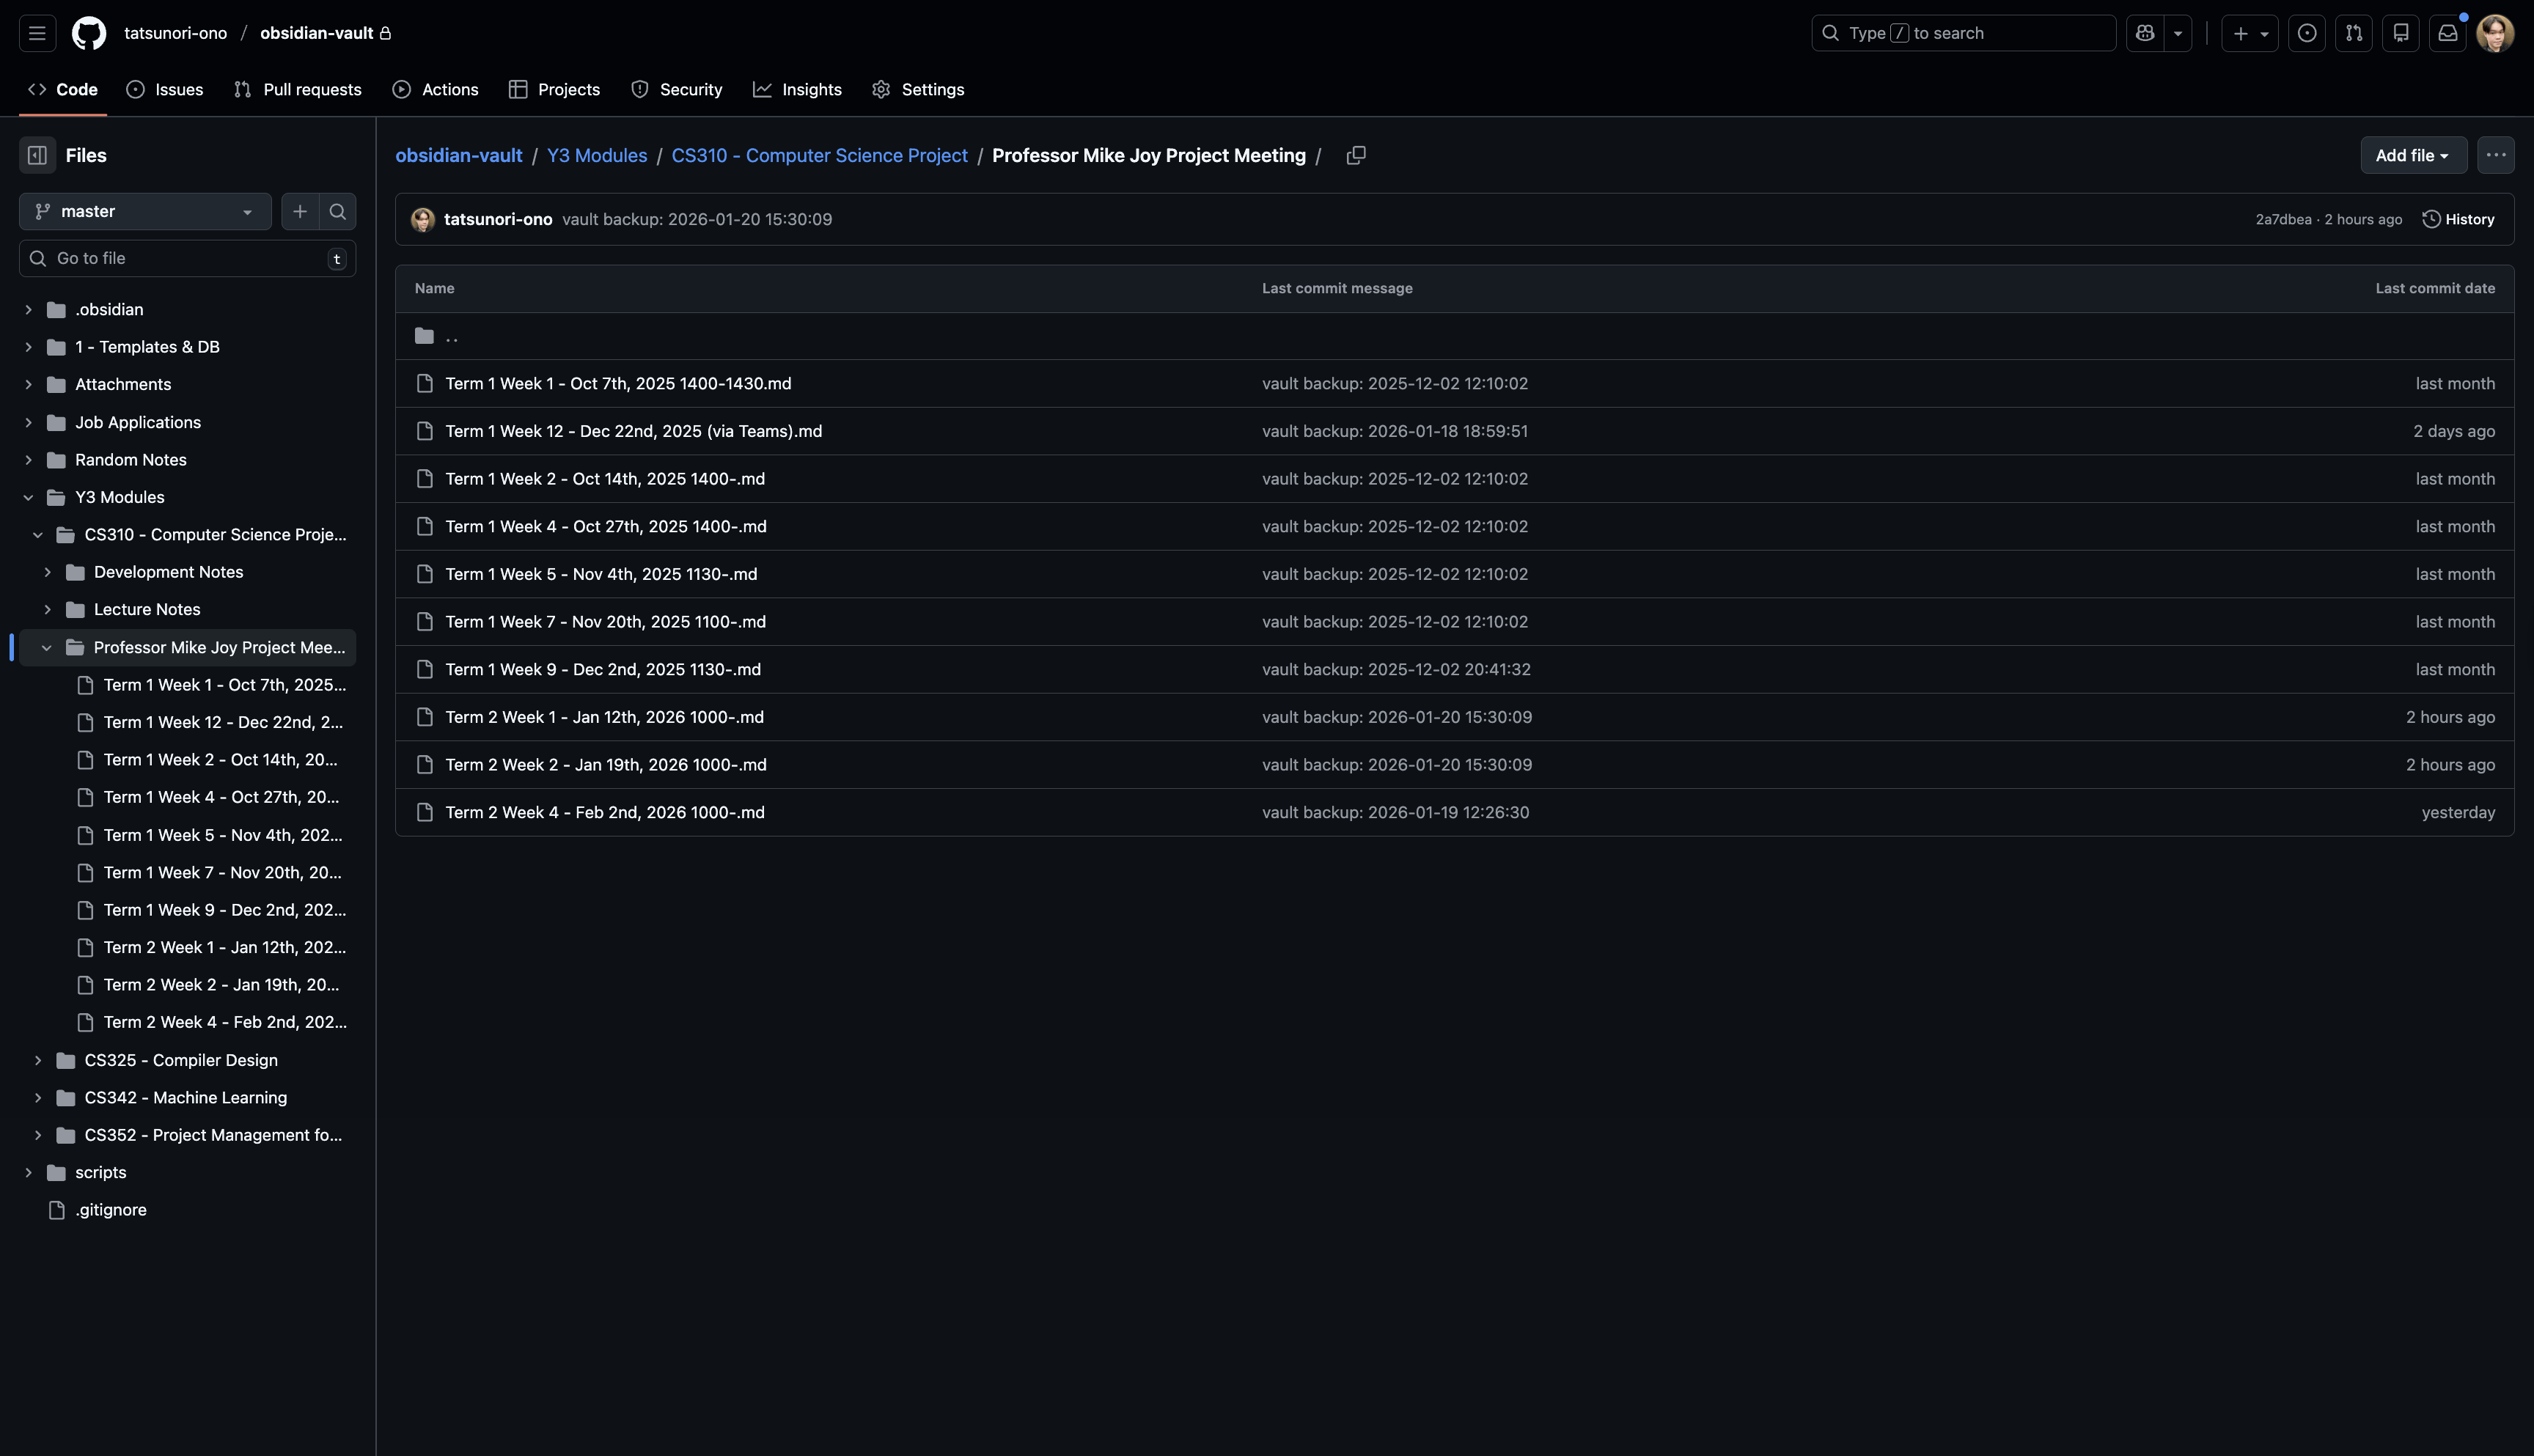
\includegraphics[width=\linewidth]{Figures/github-backup.png}
  \caption{Supervisor meeting notes backed up on GitHub every 15 minutes
           (if any changes are made).}
  \label{fig:github-backup}
\end{figure}

\section{Sample Supervision Meeting Note}
\label{appx:meeting-note}

The following screenshot shows a representative supervision meeting note in
Obsidian, using the Cornell-inspired three-section structure described in the
main body. Questions are recorded before the meeting; answers and action items
are filled in during and after.

\begin{figure}[H]
  \centering
  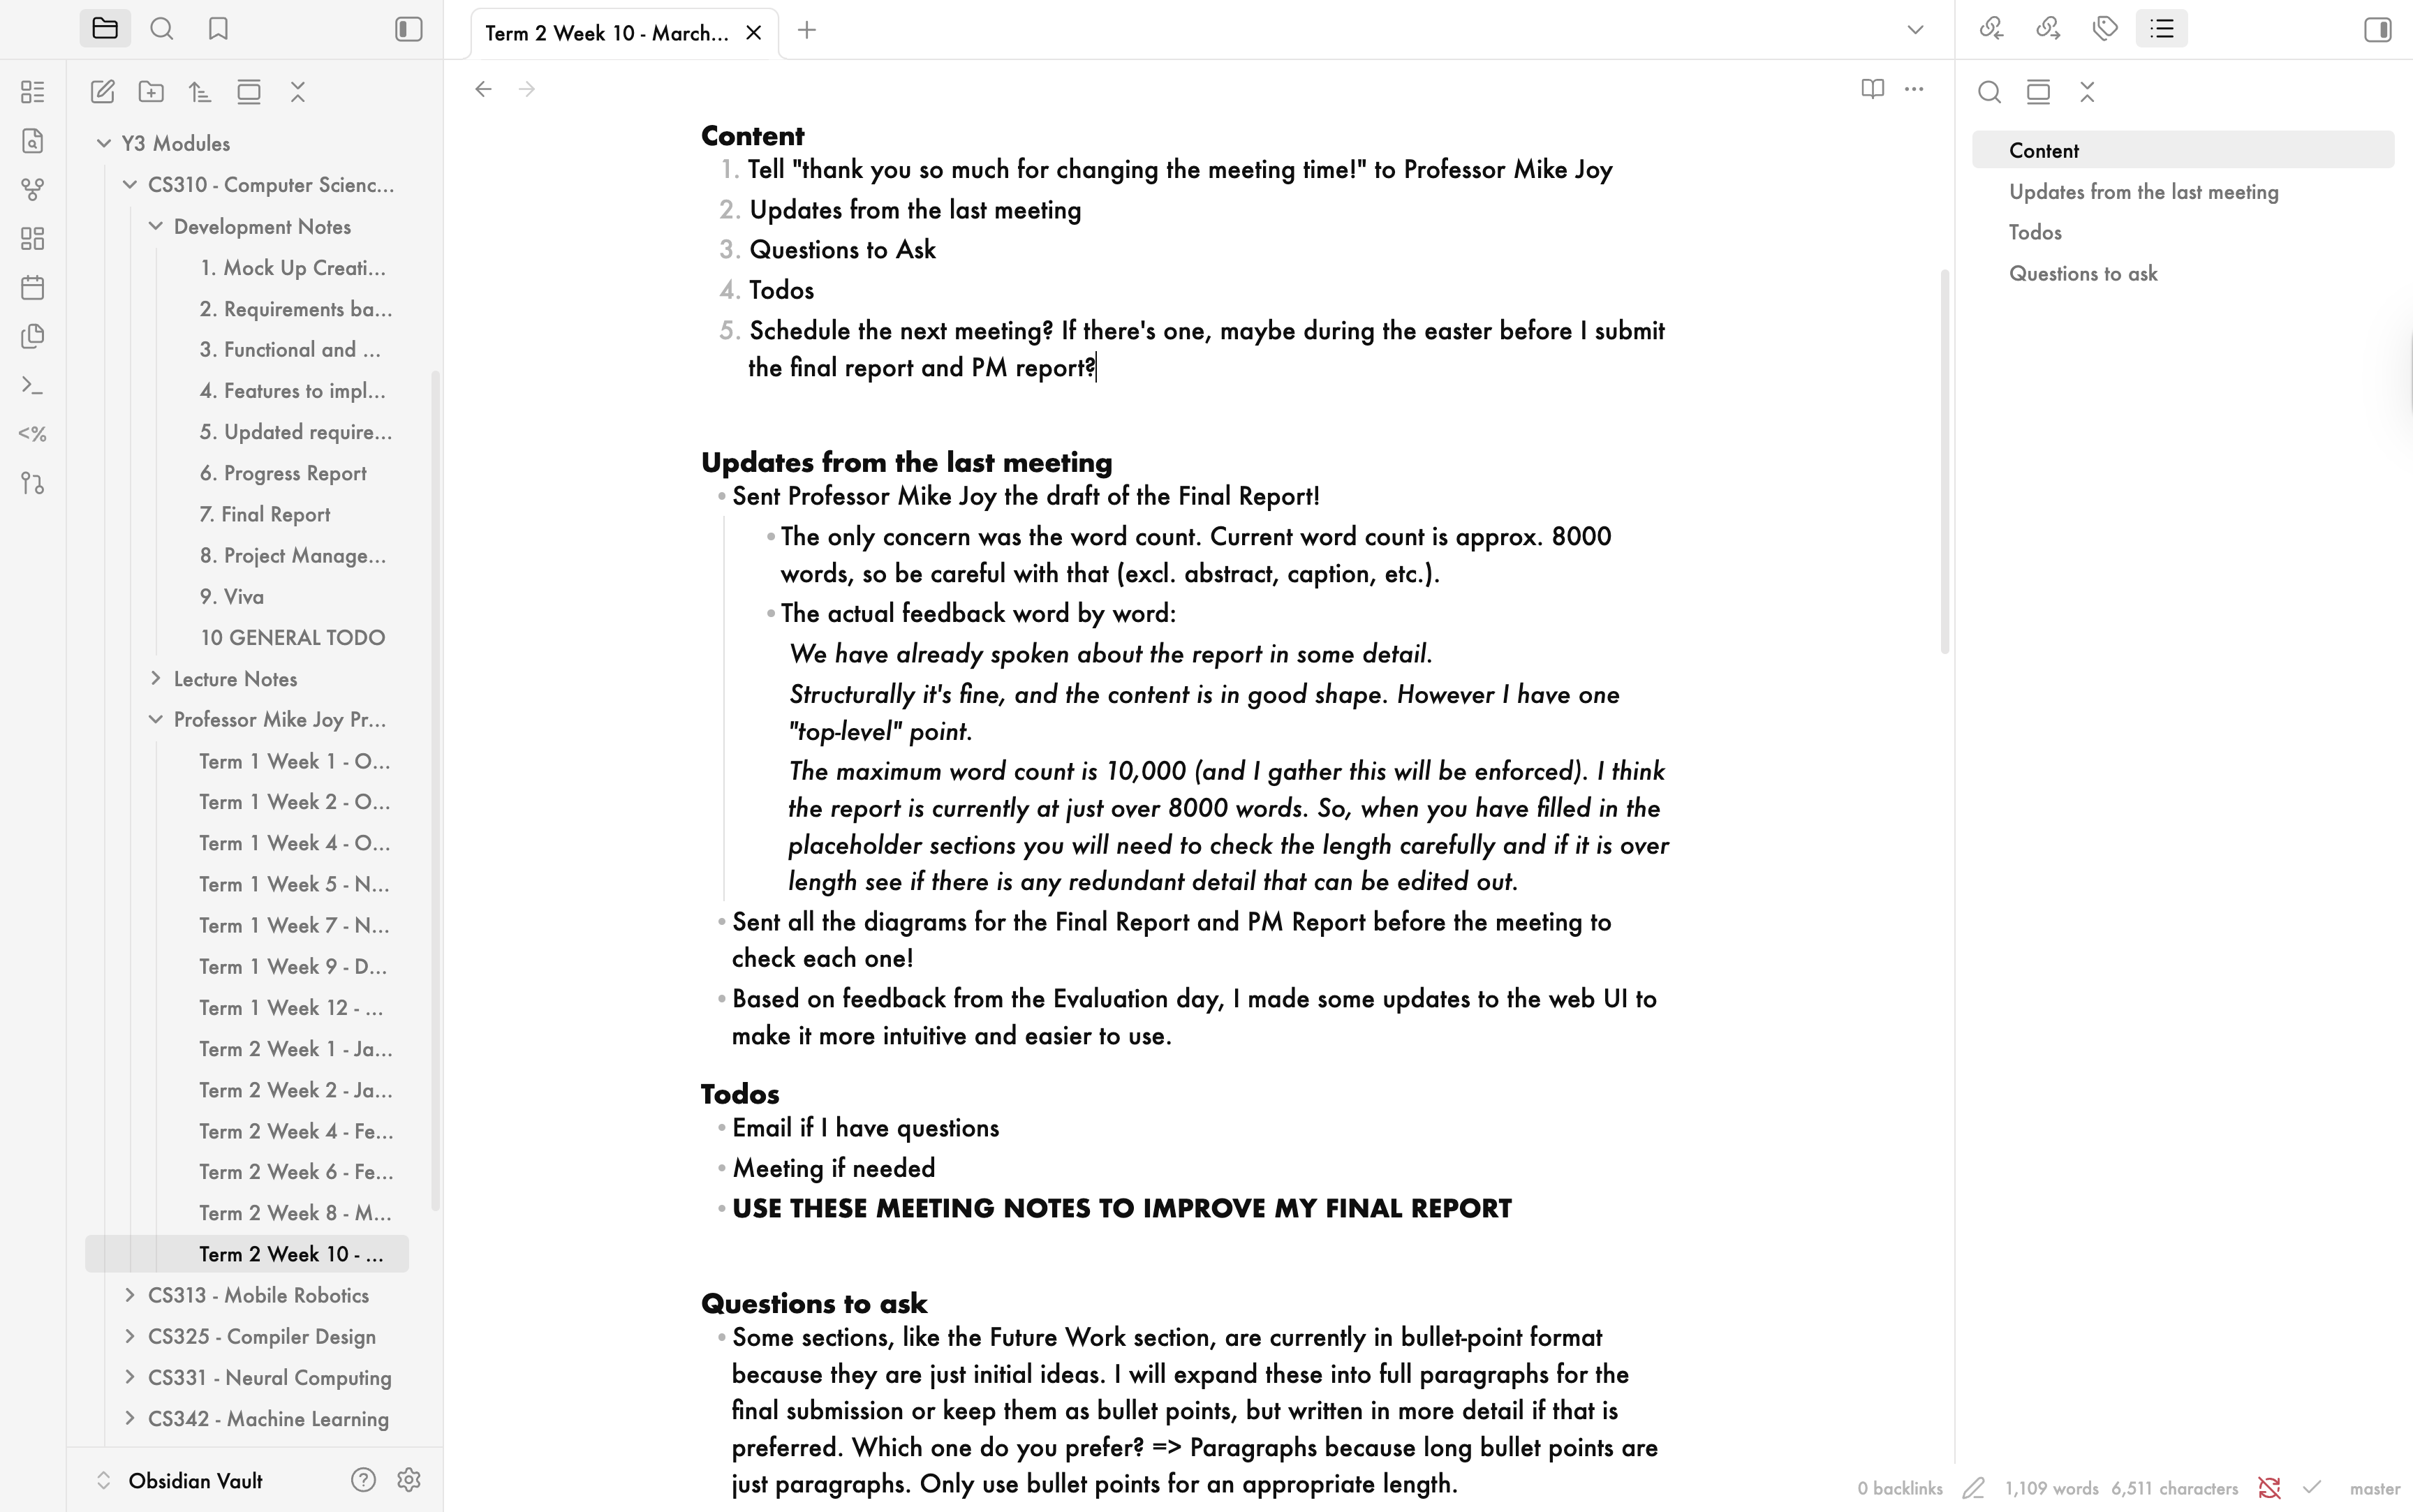
\includegraphics[width=\linewidth]{Figures/meeting-note-sample.png}
  \caption{Sample supervision meeting note in Obsidian (Cornell-inspired structure).}
  \label{fig:meeting-note}
\end{figure}

\end{appendices}

\end{document}